%%%%%%%%%%%%%%%
% implementace

\chapter{Implementace}

Většinu projektu jsem implementoval pod systémem Ubuntu Linux.
Pro vytvoření okna pod Linuxem je použita knihovna SDL.
U systému Windows je to WINAPI.
Pro spuštění programu je vyžadováno OpenGL minimálně ve verzi 3.3.
Program jsem ladil pro Windows 7.
Verze pro Linux neobsahuje hudbu a je také větší.
Důvod je ten, že knihovna pro přehrávání hudby byla napsána pro systém Windows.
Také komprimační program kkrunchy slouží pro komprimování binárních spustitelných souborů systému Windows.

%%%%%%%%%%%%%%%%%%%%
% hudba

\section{Hudba}

Pro přehrávání hudby v intru jsem použil knihovnu libv2 od německé skupiny Farbrausch \cite{V2}.
Ke knihovně je dodáván i příklad přehrávače souborů v2m.
Přehrávač byl napsán v jazyce C pro Visual Studio.
Některé části kódu byly napsány v jazyce assembler a ty bylo nutné přepsat.
Pro skládání hudby je ke knihovně přidán i VSTi plugin, zobrazen na obrázku \ref{fig:vsti}.
Hudbu jsem skládal v demo verzi programu FL Studio \cite{FLS} a použil jsem tento VSTi plugin.

\begin{figure}[h]
\centering
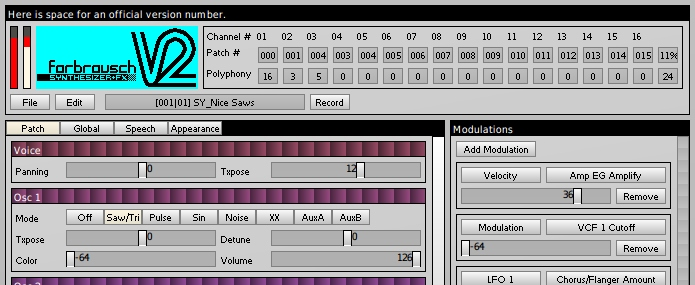
\includegraphics[width=15cm,keepaspectratio]{obr/vsti.jpg}
\caption{VSTi plugin pro tvorbu hudby pro knihovnu libv2.}
\label{fig:vsti}
\end{figure}



%%%%%%%%%%%%%%%%%%%
% scene

\section{Scény intra}
Intro obsahuje čtyři scény.
Horskou scénu, přímořskou scénu, tunel a jeskyni.
Mezi scénami je plynule přepínáno pomocí zatmívaček.
Zatmívačka je černá plocha.
Tato plocha je kreslena s vypnutým hloubkovým testem.
Ovlivňováním průhlednosti můžeme plynule přejít mezi scénami.
V intru se vyskytují tyto objekty: hory, kopce, skybox, vodní hladina, vodopády, bublinky ve vodě, 
chomáče rostlin, liánové rostliny, bedny, tunel, jeskyně a zavěšené barevné koberce.
\subsection{Horská scéna}
Scéna s horskou scénou je na obrázku \ref{fig:hory}.
Pro vytvoření terénu je použita výšková mapa.
Výšková mapa je vytvořena ze vzdálenostního pole Voroného diagramů, pravá strana ob\-ráz\-ku \ref{fig:voronoid}.
Ve vzdálenostním poli se vyskytují špičky (horské štíty) a propoje (hřebeny).
Na hory je namapována bump mapa, která vytváří skály.
Barva hor je vytvořena dvojicí barevných přechodů.
Jeden barevný přechod je použit stejným způsobem jako na obrázku \ref{fig:gradmap}.
Tímto způsobem získáme barvu s nadmořskou výškou.
Druhý barevný přechod je použit pro obarvení srázů.
Výběr barvy z přechodu je stejný jako u prvního přechodu - pomocí výšky.
Barva je ale přimíchávána pomocí průhlednosti.
Průhlednost je určena podle strmosti srázu - podle normály $n=(u,v,w)$.
Pokud je složka $|v|=1$ je průhlednost maximální.
Při $|v|=0$ je průhlednost minimální.
Kolem hor je skybox, který je zobrazen na obrázku \ref{fig:skybox0}.
S rostoucí vzdáleností se hory noří do mlhy.
Hustota mlhy je vyšší s menší nadmořskou výškou.
\begin{figure}[h]
\centering
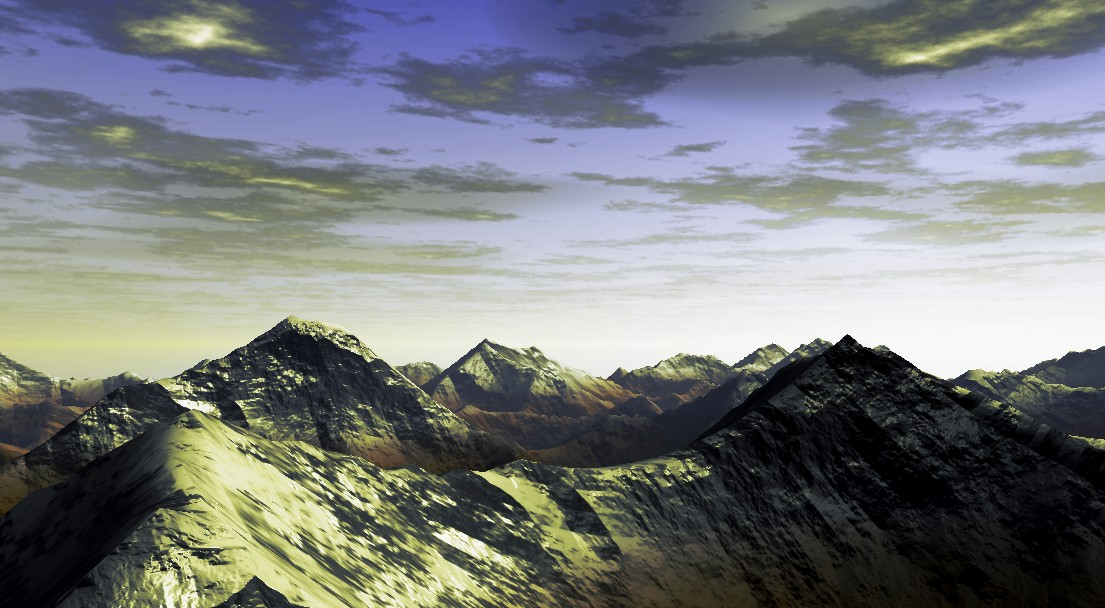
\includegraphics[width=15cm,keepaspectratio]{obr/hory0.jpg}
\caption{Horská scéna.}
\label{fig:hory}
\end{figure}

\subsection{Přímořská scéna}
Přímořská scéna zobrazena na obrázku \ref{fig:pobrezi} je vytvořena pomocí výškové mapy vytvořené ze šumu.
Stejně jako u hor, jsou pro obarvení použity dva barevné přechody.
Skybox kolem přímořské oblasti můžeme vidět na obrázku \ref{fig:skybox1}.
\begin{figure}[h]
\centering
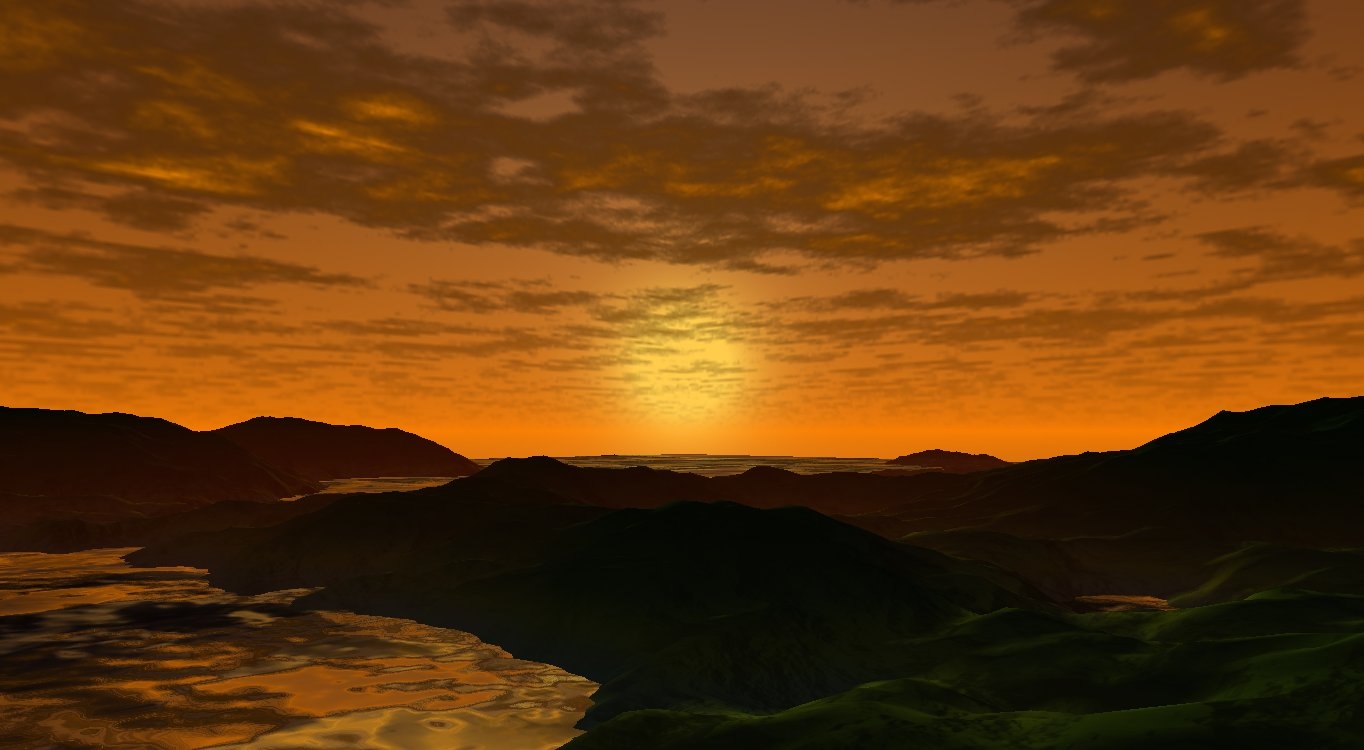
\includegraphics[width=15cm,keepaspectratio]{obr/pobrezi.jpg}
\caption{Přímořská scéna.}
\label{fig:pobrezi}
\end{figure}

\subsection{Tunel, jeskyně}
Tunel i jeskyně jsou vytvořeny stejným způsobem, pomocí algoritmu Marching Tetrahedra.
Rozdíl spočívá ve vytvoření trojrozměrného pole volumetrické reprezentace.
U jeskyně je způsob vytvoření pole jednoduchý.
Vygenerujeme trojrozměrný šum pomocí algoritmu půlení intervalu.
Šum poté vyhladíme pomocí globální transformace.
Poté budeme hodnoty pole násobit koeficientem $k=\langle 0,1 \rangle$.
Hodnota koeficientu $k$ klesá, pokud se vzdalujeme od středu krychle obsahující šum.
Tímto zajistíme, aby se jeskyně uzavřela a neměla ve stěnách díry.
Výslednou objemovou reprezentaci jeskyně převedeme pomocí algoritmu Marching Tetrahedra na trojúhelníky.

Objemová reprezentace tunelu je vytvořena jiným způsobem.
Nejprve vytvoříme troj\-roz\-měr\-ný šum stejně jako u jeskyně.
Hodnoty šumu zmenšíme tak, aby nebyly větší než práh pro algoritmus Marching Tetrahedra.
Pokud bychom teď provedli převod na trojúhelníky, žádný trojúhelník by nevznikl.
Nyní do pole vykreslíme tunel.
Tunel budeme vykreslovat po bodech.
Body leží na křivce podobné jednomu vláknu blesku.
Konce křivky umístíme na opačné rohy krychle šumu.
Křivka je reprezentována dvěma jednorozměrnými šumy.
Jeden ovlivňuje natočení kolem spojnice počátečního a koncového bodu křivky.
Druhý ovlivňuje vzdálenost od spojnice.
Tuto křivku vykreslíme do pole několikrát a vznikne nám tak tunel zobrazený na obrázku \ref{fig:tunel}

Textury v tunelu jsou rozmístěny stejně jako v jeskyni.
Jeskyně je obarvena pomocí několika textur: Textury stropu, textury stěn a textury země.
Každá z těchto textur má k sobě i bump mapu.
Další textura je jednorozměrná a je umístěna vertikálně.
Představuje geologické vrstvy.
Další textura je trojrozměrná.
Je vytvořena pomocí distančního pole z Voroného diagramů a reprezentuje kaustiky.
Textura je trojrozměrná, abychom mohli kaustiky animovat.
Poslední textura je také trojrozměrná a je dynamicky měněna.
Před\-sta\-vu\-je vlhkost stěn jeskyně.
Vodopády do ní zapisují hodnoty a textura samotná ovlivňuje míru odlesků a tmavost povrchu.

V tunelu jsou umístěny chomáče rostlin.
Jedná se o částicový systém, jehož částice jsou statické.
Textura částic je zobrazena v levé části obrázku \ref{fig:listy}.
Na konci tunelu je vodní hladina.
V tunelu se vyskytuje i pavučina.
Pavučina je složena z elastického systému	a můžeme ji vidět uprostřed obrázku \ref{fig:tunel}.

V jeskyni jsou zavěšeny liánové rosliny.
Rostliny jsou složeny z elastického systému, jehož tvar je v pravé části obrázku \ref{fig:listy}.
Jeden článek rostliny je složen ze dvou spojených čtyřstěnů.
V bodech je umístěna textura rosliny zobrazena v levé části obrázku \ref{fig:listy}.
Dalším objektem jeskyně je zavěšený koberec.
Koberec je také složen z elastického systému ve tvaru mřížky.
Na koberec je nanesena textura na obrázku \ref{fig:koberec}

\begin{figure}[h]
\centering
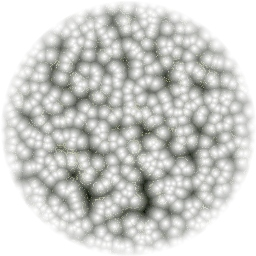
\includegraphics[width=3cm,keepaspectratio]{obr/listy.jpg}
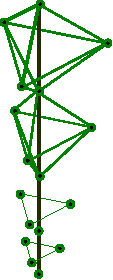
\includegraphics[width=2cm,keepaspectratio]{obr/liana.pdf}
\caption{Vlevo: textura rostlin.
Vpravo: rozložení uzlů a spojů elastického systému liánové rostliny.}
\label{fig:listy}
\end{figure}

\begin{figure}[h]
\centering
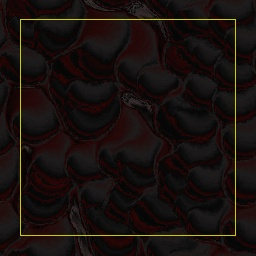
\includegraphics[width=4cm,keepaspectratio]{obr/koberec.jpg}
\caption{Textura zavěšeného koberce.}
\label{fig:koberec}
\end{figure}

\begin{figure}[h]
\centering
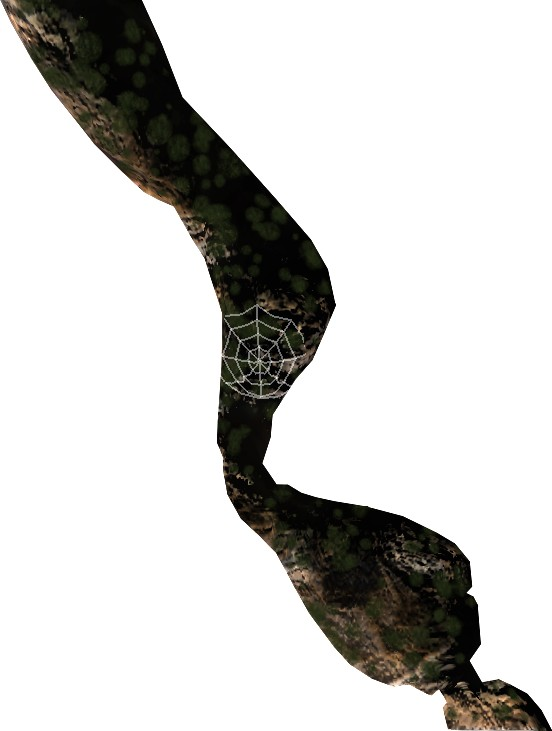
\includegraphics[width=7.5cm,keepaspectratio]{obr/tunel.jpg}
\caption{Tunel.}
\label{fig:tunel}
\end{figure}

\begin{figure}[h]
\centering
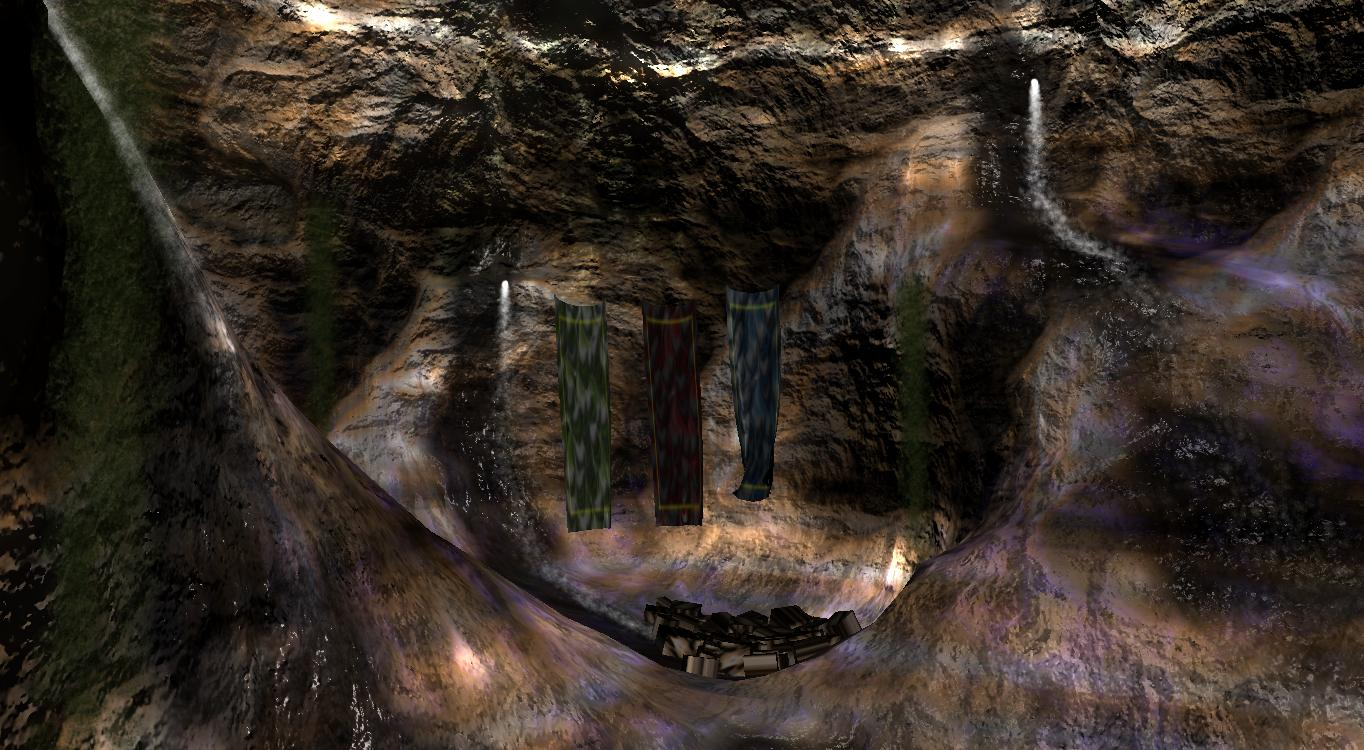
\includegraphics[width=15cm,keepaspectratio]{obr/jeskyne.jpg}
\caption{Jeskyně.}
\label{fig:jeskyne}
\end{figure}








%%%%%%%%%%%%%%
% glsl

\section{GLSL}

V intru jsem použil sedm shader programů.
Tři z nich používají i geometry shader.
Jsou to shader programy využívané částicovými systémy.
O vytvoření částice (plošky) se stará geometry shader.
Pro částicové systémy je vyhrazen vlastní shader program.
Pomocí uniformu lze nastavit, jestli se částice natáčí ke kameře či udržuje svoji orientaci.

Shader program, který v intru používáme pro vykreslení jeskyně má nejsložitější část fragment shader.
Jeskyně obsahuje poměrně malé množství trojúhelníků a přesto je nej\-slo\-ži\-těj\-ší na vykreslení.
Snížením počtu trojúhelníků bychom složitost nesnížili.
Jednou možností je optimalizovat fragment shader.
Vhodnou optimalizací může být minimalizace větvení programu použitím vestavěných funkcí.
Příklad větvení:
\begin{verbatim}
if (red_flag == 1){
  color = vec3(1,0,0);
}else{
  color = texture(wall,coord);
}
\end{verbatim}
Výše uvedený úsek programu obsahuje větvení pomocí uniformu $red\_flag$.
Můžeme se větvení zbavit využitím vestavěné funkce $mix$.
\begin{verbatim}
color=mix(vec3(1,0,0),texture(wall,coord),red_flag);
\end{verbatim}
Další funkce, které se dají použít pro odstranění větvení jsou $min,max,clip,clamp$ a další.
Jinou možností je omezení používání množství normalizační funkce: $normalize$.
Urychlení vykreslení scény se složitým fragment shaderem můžeme udělat i jinak.
Urychlení spočívá v omezení množství fragmentů, které musíme vykreslit.
Při vykreslování se stává, že jsou trojúhelníky kresleny ve špatném pořadí.
Vykreslujeme některé fragmenty, které jsou později přepsány novými hodnotami.
Řešení může existovat v algoritmu řazení trojúhelníků.
Potom stačí vykreslovat od nejbližších trojúhelníků.
V případě, že je nějaká část trojúhelníku zakryta, je vykreslování zastaveno hloubkovým testem.
Řazení trojúhelníků je ale složité na výpočet a zbytečně by nám zabralo místo v programu.
Jeskyně ale obsahuje málo trojúhelníků, proto vykreslíme nejprve hloubkový buffer s vypnutým zápisem barvy.
Tím se přeskočí část s fragment shaderem.
Poté vykreslíme scénu znovu, tentokrát již s povoleným zápisem barvy.
Tímto zajistíme, že se výpočet fragment shaderu provádí jen pro nezbytně nutné množství fragmentů.



%%%%%%%%%%%%%%%%%%%%
% rozdeleni

\section{Rozdělení projektu a FPS}
Zdrojové kódy přesahují 20 000 řádků kódu, proto je bylo potřeba kvůli přehlednosti rozdělit do logických celků.
Projekt je rozdělen do velkého množství knihoven.
Ve zdrojových kódech pro Linux jsou knihovny rozděleny do několika složek:
\begin{description}

\item[app] V této složce jsou funkce pro obsluhu vytvoření okna a časování.
\begin{description}
\item[winwindow] Knihovna obsahuje funkce pro vytvoření okna, nastavení obslužných funkcí.
Dále obsahuje řízení časem.
Knihovna je preprocesorem rozdělena do dvou částí.
Jedna část je pro systém Windows 7 a obsahuje kód ve WINAPI.
Druhá část je pro systém Linux a využívá funkcí knihovny SDL.
\item[main] Obsahuje hlavní část programu, většinu inicializací a krokování.
Obsahuje kreslící funkci.
\end{description}

\item[adt] Složka obsahuje abstraktní datové typy.
\begin{description}
\item[list2] Obsahuje obecný dvousměrný seznam.
\item[relist] Reprezentuje obecné pole s automatickým zvětšování velikost.
Oproti {\bf list2} je rychlejší čtení, ale pomalejší vkládání doprostřed pole.
\item[ntree] Představuje obecný strom a obslužné funkce.
\item[adtfce, adt] Obsahují rozhraní a funkce společné pro abstraktní datové typy.
\end{description}

\item[elastic] Složka obsahuje pouze jednu knihovnu, která implementuje elastický systéme a jeho obslužné funkce

\item[enviroment] Ve složce nalezneme knihovny pro grafické objekty intra.
\begin{description}
\item[box\_swarm] Knihovna obsahuje funkce pro inicializaci, umístění, vykreslení a pře\-po\-čí\-tá\-ní haldy beden.
\item[bubble] Knihovna obsahuje částicový systém reprezentující bublinky ve vodě.
\item[carpet] Objekt zavěšeného koberce je obsahem této knihovny.
\item[cave] Obsahuje funkce pro vygenerování jeskyně.
\item[collide] Obsahuje kolizní systém.
\item[fade] Zatmívačka, která slouží pro přechod mezi scénami
\item[font] Obsahuje funkce a font pro vykreslení textu.
\item[geometry] V knihovně můžeme najít funkce pro výpočet normál a výpočet spojů pro elastický systém.
\item[lake] Vodní hladina a obslužné funkce jsou obsaženy v této knihovně.
\item[moss] Obsahem knihovny je objekt mechu nebo křoví.
\item[mountain, waterside] Obsahují funkce pro vytvoření výškových map hor a přímořských kopců.
\item[object] Soubory knihovny reprezentují obecný objekt, který využívá elastický systém.
\item[particle] Nalezneme zde obecný částicový systém, který je využíván například v knihovně {\bf bubble}.
\item[plant] Rostlina složená z elastického systému.
\item[skybox] Obsahuje funkce pro vykreslení skyboxu.
\item[skyboxgenerate] Vytvoření skyboxu je součást funkcí v souborech této knihovny.
\item[spiderweb] Knihovna reprezentuje pavučinu.
\item[terrain] Vykreslení a vytvoření geometrie terénu pomocí výškových map.
\item[tunnel] Obdobně jako {\bf cave} obsahuje knihovna funkce pro vygenerování tunelu.
\end{description}

\item[gen] Složka obsahuje některé obecné algoritmy pro generování.
\begin{description}
\item[color] Obsahuje funkce pro práci s HSV barevným modelem.
\item[map, colormap] Funkce pro práci s barevným přechodem.
\item[midpoint] Algoritmus pro generování šumu pomocí půlení intervalu.
\item[voronoi] Generování Voroného diagramů.
\end{description}

\item[gpu] Složka obsahuje knihovny pro komunikaci s grafickou kartou.
\begin{description}
\item[gpuattribute] Funkce pro práci s atributy shader programu.
\item[gpubuffer] Obsahuje funkce pro správu bufferů na grafické kartě.
\item[gpushaderprogram] Obsahuje obslužné funkce pro shader programy.
\item[gputexture] Inicializace a správa textur.
\item[gputextureunit] Obsluha texturovacich jednotek.
\end{description}

\item[index] Knihovny pro práci s vícerozměrnými daty.
\begin{description}
\item[index] Knihovna obsahuje obecný $d$ dimenzionální index.
\item[nsize] Rozměry $d$ dimenzionálních dat.
\end{description}

\item[marchingtetra] Složka obsahuje algoritmus Marching tetrahedra.
\begin{description}
\item[mt\_core] Algoritmus Marching tetrahedra.
\item[pack] Algoritmus pro spojování společných vrcholů trojúhelníků.
\end{description}

\item[music] Složka obsahuje přehrávač a hudební soubory.
\begin{description}
\item[music] Funkce pro inicializace a přehrání hudby.
\item[songs] Hudební skladby.
\item[v2mplayer] Přehrávač hudby.
\end{description}

\item[mymath] Složka obsahuje matematické knihovny.
\begin{description}
\item[camera] Kamera scény.
\item[cameracontrol] Systém pro pohyb kamery.
\item[vector, matrix] Operace s vektory a maticemi.
\item[stdmath] Základní matematické vztahy.
\item[transform] Transformace scény.
\end{description}

\item[mymem] Složka obsahuje knihovnu pro práci s pamětí a zastřešuje rozdíly mezi systémy Windows a Linux.
\item[shaderprogram] Obsahem složky jsou vertex, geometry a fragment shadery.
\item[std] Základní funkce.
Funkce pro generování náhodného čísla.
Funkce pro zobrazení grafu načítání. 

\item[texturefactory] Složka obsahuje knihovny pro generování textur.
\begin{description}
\item[colorbuffer] Obsahuje funkce pro práci s $d$ rozměrnými poli pro vytvoření textur.
\item[convolution] Obsahuje $d$ rozměrnou konvoluci.
\item[fastgetvalue] Obsahuje obtimalizované funkce pro přístup k $d$ rozměrným polím.
\item[globaltransform] Obsahuje globální transformační funkce pro tvorbu textur.
\item[localtransform] Obsahuje lokální transformační funkce pro tvorbu textur.
\end{description}



\end{description}


\newpage
\subsection{FPS}

V grafu zobrazeném na obrázku \ref{fig:fps} můžeme vidět průběh počtu snímku za sekundu (FPS) v čase.
V prvních dvou částech grafu FPS hodně kolísá.
V ostatních částech FPS udržuje přibližně konstantní hodnotu.
První dvě scény zobrazují horskou a přímořskou krajinu.
Každá z těchto scén je složena z 130 050 trojúhelníků.
Záleží proto na pozici a záběru kamery, jak velká bude hodnota FPS.
Lokální maxima poukazují na místa v intru, kde kamera zabírá jen zlomek scény.
Příkladem může být špička v druhé scéně.
V přímořské oblasti se kamera chvíli dívá jen na skybox. 
To vysvětluje velký nárůst FPS.
V posledních dvou scénách: tunelu a jeskyně je řádově méně trojúhelníků.
Proto tolik nezávisí na záběru kamery.
První dvě scény jsou náročnější z pohledu množství trojúhelníků.
Poslední dvě scény pak z pohledu shader programu, který je složitější.

\begin{figure}[h]
\centering
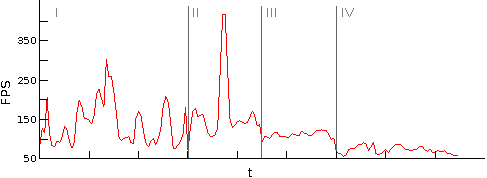
\includegraphics[width=15cm,keepaspectratio]{obr/fps.pdf}
\caption{Průběh počtu snímku za sekundu v čase.
Graf je rozdělen do čtyř částí podle scén.}
\label{fig:fps}
\end{figure}
